\documentclass[a4paper, 12pt]{article}
\usepackage{titling}
\usepackage{array}
\usepackage{booktabs}
\usepackage{enumitem}
\usepackage{graphicx}
\usepackage{hyperref}
\usepackage{amssymb}
\usepackage{listings}
\usepackage{color} %red, green, blue, yellow, cyan, magenta, black, white
\setlength{\heavyrulewidth}{1.5pt}
\setlength{\abovetopsep}{4pt}
\setlength{\parindent}{0pt}
\graphicspath{{.}}

\usepackage[margin=1in]{geometry}
\definecolor{mygreen}{RGB}{28,172,0} % color values Red, Green, Blue
\definecolor{mylilas}{RGB}{170,55,241}
% Must be after geometry
\usepackage{fancyhdr}
\pagestyle{fancy}
\fancyhf{}
\rhead{NN Homework 2}
\lhead{P.Lukin, I. Vishniakou, E. Ovchinnikova}
\cfoot{\thepage}

\setlength{\droptitle}{-5em}

\title{Neural Networks  \\
				- Homework 2 -}
\author{Petr Lukin, Ivan Vishniakou, Evgeniya Ovchinnikova}
\date{Lecture date: 10 October 2016}

\begin{document}

%-------------------------------------------------------------------------------
\lstset{language=Matlab,%
    %basicstyle=\color{red},
    breaklines=true,%
    morekeywords={matlab2tikz},
    keywordstyle=\color{blue},%
    morekeywords=[2]{1}, keywordstyle=[2]{\color{black}},
    identifierstyle=\color{black},%
    stringstyle=\color{mylilas},
    commentstyle=\color{mygreen},%
    showstringspaces=false,%without this there will be a symbol in the places where there is a space
    numbers=left,%
    numberstyle={\tiny \color{black}},% size of the numbers
    numbersep=9pt, % this defines how far the numbers are from the text
    emph=[1]{break},emphstyle=[1]\color{red}, %some words to emphasise
    %emph=[2]{word1,word2}, emphstyle=[2]{style},
}

%-------------------------------------------------------------------------------

\maketitle

\section{Mind map}

\begin{figure}[h]
  \centering
  \caption{S. Haykin, Neural Networks, chapter 2 (before 2.13). Mind map (a zoomed version of the map is attached as mindmap.png file).\label{fig:mindMap}}
  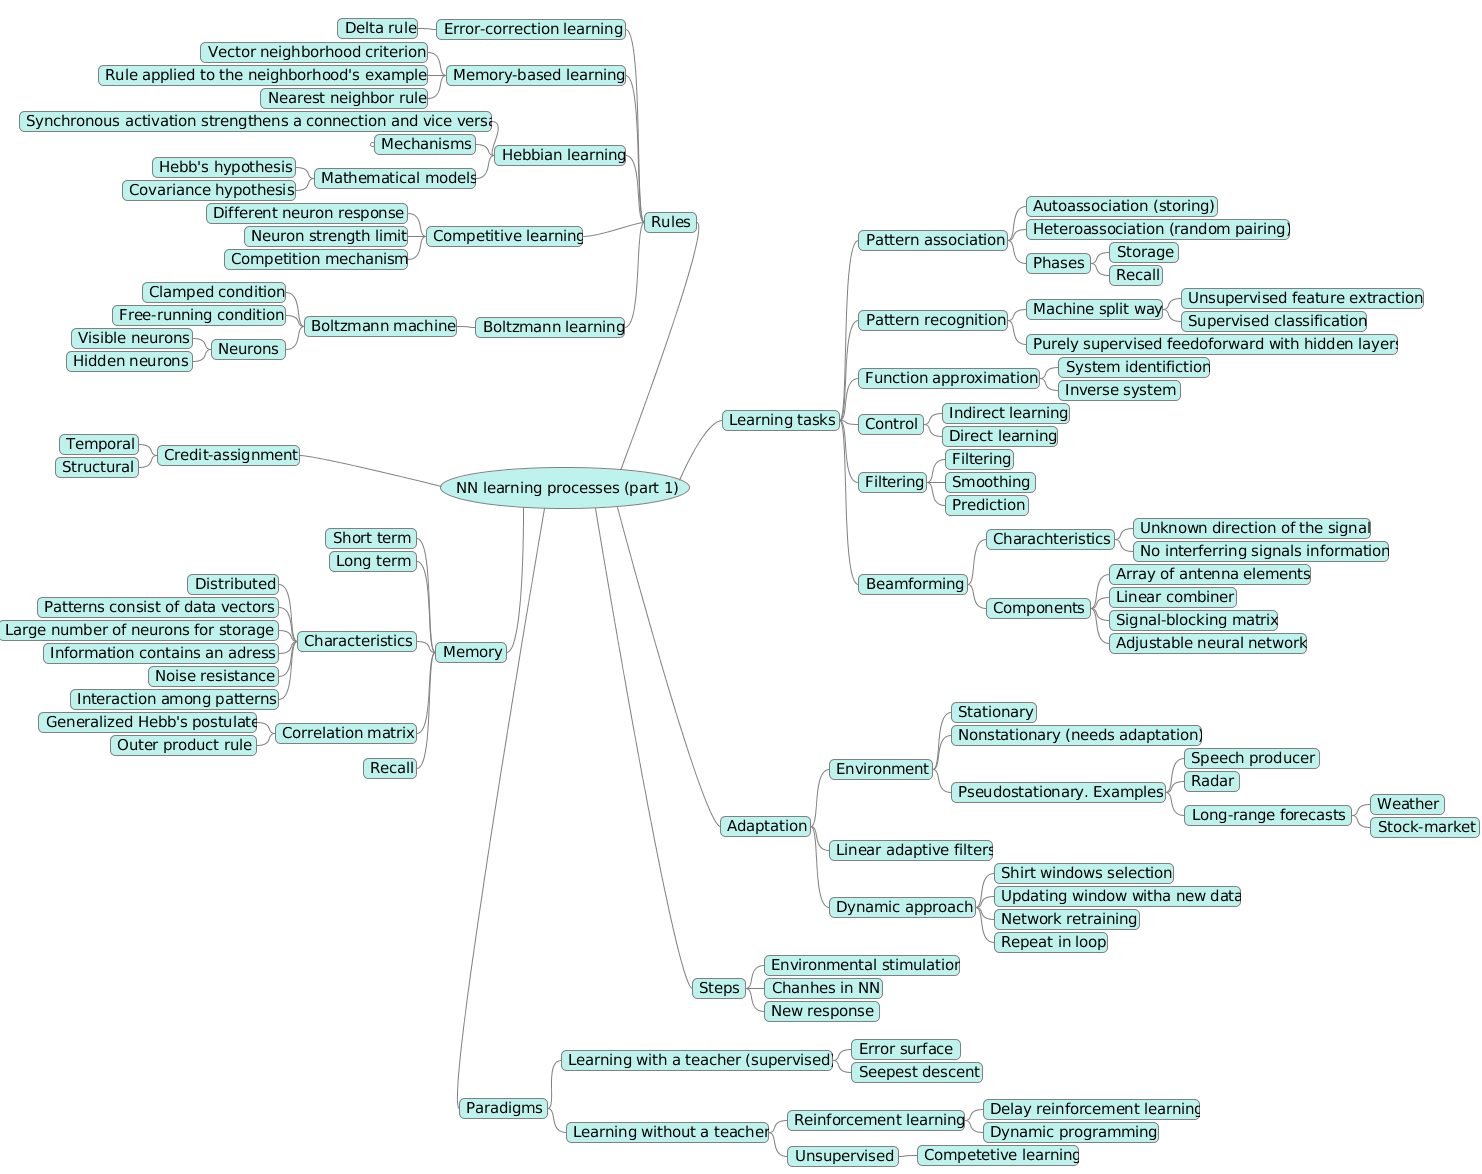
\includegraphics[width=1.0\textwidth]{mindmap}
\end{figure}

\newpage
\section{Exercises}

\subsection{Exercise 1.13}

Do the problem 1.13 (Network architecture) from the previous week�s assignment. This time use MATLAB or Python�s (sympy) symbolic toolbox. Finally assume the network presented in fig P1.13 is a binary-classifier, please depict how the input space (R2) is classified on a 2D graph using different colors.

\medskip

This exercise was solved in matlab. The input-output mapping can be made for a network with structure $2-2-..-2-1$ with different weights and squashing functions: linear, sigmoid. Output layer also can have heaviside squashing function.

\medskip

The network itself has a following structure:
\medskip


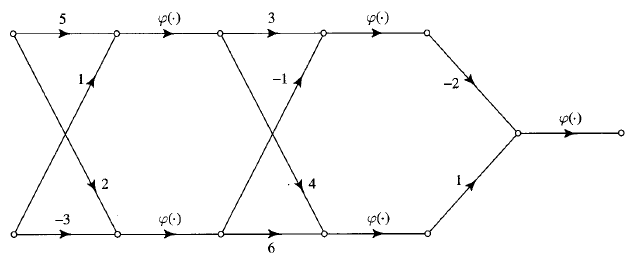
\includegraphics[scale=0.7]{113.png}


\medskip
Here is the code of the hidden layer output implementation.
\medskip

\lstinputlisting{hiddenlayer.m}

The output layer.


\lstinputlisting{outputlayer.m}

Mapping calculation and plotting.


\lstinputlisting{ex113.m}

Plots of the input-output mappings.

Sigmoid squashing function:
\begin{center}
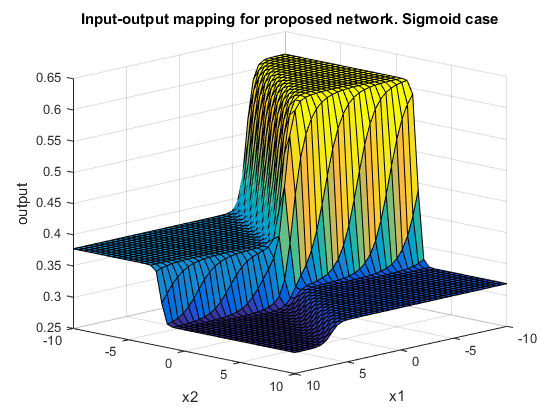
\includegraphics[scale=0.8]{sigmoid.png}
\end{center}

Linear squashing function:
\begin{center}
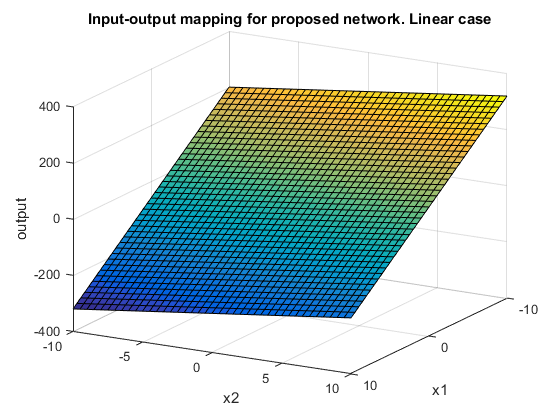
\includegraphics[scale=0.8]{linear.png}
\end{center}

Binary classifier:
\begin{center}
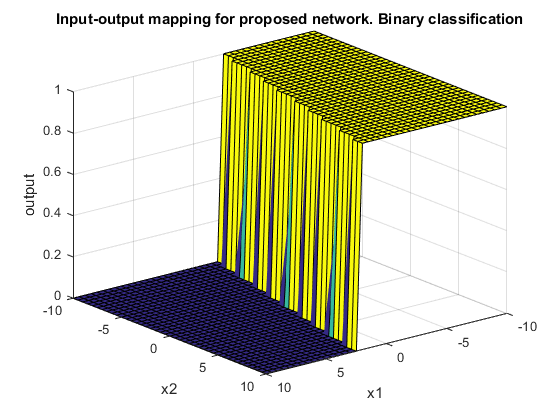
\includegraphics[scale=0.8]{classification.png}
\end{center}

\subsection{Exercise 4}

Derive the Delta rule for two ADALINE neural networks depicted in Fig. \ref{fig:nn1}, Fig. \ref{fig:nn2}.

Solution:\\

1 neural network.\\

\begin{figure}[h]
  \centering
  \caption{Neural network 1. \label{fig:nn1}}
  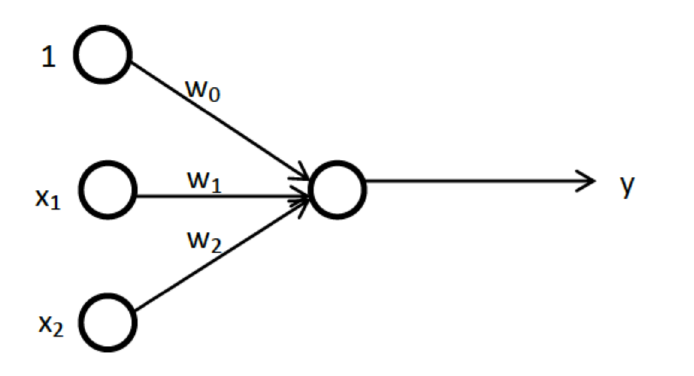
\includegraphics[width=0.5\textwidth]{nn1}
\end{figure}

Input: 	$\vec{x} = (x_0, x_1, x_2)$,  where $x_0 = 1$\\
Weights: 	$\vec{w} = (w_0, w_1, w_2)$\\
Output: $y = \vec{x} \vec{w} = w_0 + x_1w_1 + x_2w_2$\\

$e = d - y = d - (w_0 + x_1w_1 + x_2w_2)$, where d is a desired value.\\

$E(w) = \frac{1}{2}e^2$\\

Each $i^{th}$ weight with an should be moved in the direction $\frac{\partial E}{\partial w_i}$:\\

$\frac{\partial E}{\partial w_i} = x_i(d - (w_0 + x_1w_1 + x_2w_2))$\\

So, each step will change each weight by the following value:\\
$\Delta w_i = \eta x_i(d - (w_0 + x_1w_1 + x_2w_2))$,\\
where $\eta$ is a learning rate that should be chosen according to the specific of the certain case. It can be either a constant (0.5, 1, etc.) or variable, or adaptive.\\

Therefore the delta rule will take the following form:\\

$w_i^{new} = w_i^{old} + \eta x_i(d - (w_0 + x_1w_1 + x_2w_2))$\\

Neural network 2.

\begin{figure}[h]
  \centering
  \caption{Neural network 2. \label{fig:nn2}}
  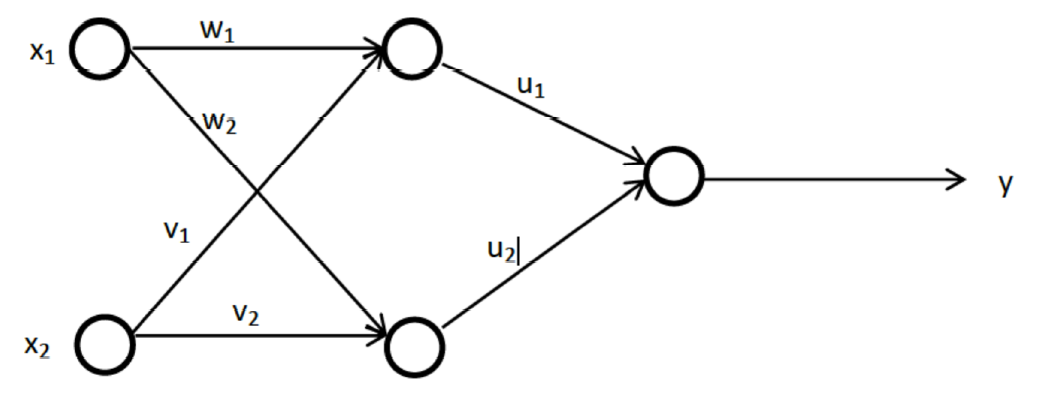
\includegraphics[width=0.6\textwidth]{nn2}
\end{figure}

Input: 	$\vec{x} = (x_1, x_2)$\\
Weights: 	$\vec{w} = (w_1, w_2)$, $\vec{v} = (v_1, v_2)$, $\vec{u} = (u_1, u_2)$\\
Activation function is linear, so:\\
Output: $y = u_1(x_1w_1 + x_2v_1) + u_2(x_1w_2 + x_2v_2)$\\

$e = d - y = d - (u_1(x_1w_1 + x_2v_1) + u_2(x_1w_2 + x_2v_2))$.\\

Each $i^{th}$ weight with an should be moved in the direction $\frac{\partial E}{\partial weight_i}$:\\

$\frac{\partial E}{\partial v_i} = x_1u_i(d - (u_1(x_1w_1 + x_2v_1) + u_2(x_1w_2 + x_2v_2))$\\

$\frac{\partial E}{\partial w_i} = x_2u_i(d - (u_1(x_1w_1 + x_2v_1) + u_2(x_1w_2 + x_2v_2))$\\

$\frac{\partial E}{\partial u_i} = (x_1w_i + x_2v_i)(d - (u_1(x_1w_1 + x_2v_1) + u_2(x_1w_2 + x_2v_2))$\\

So, each step will change each weight by the following value:\\

$\Delta w_i = \eta_w x_1u_i(d - (u_1(x_1w_1 + x_2v_1) + u_2(x_1w_2 + x_2v_2))$,\\
$\Delta v_i = \eta_v x_2u_i(d - (u_1(x_1w_1 + x_2v_1) + u_2(x_1w_2 + x_2v_2))$\\
$\Delta u_i = \eta_u (x_1w_i + x_2v_i)(d - (u_1(x_1w_1 + x_2v_1) + u_2(x_1w_2 + x_2v_2))$\\

Therefore the delta rule will take the following form:\\

$w_i^{new} = w_i^{old} + \eta x_i(d - (w_0 + x_1w_1 + x_2w_2))$\\
$v_i^{new} = v_i^{old} + \eta_v x_2u_i(d - (u_1(x_1w_1 + x_2v_1) + u_2(x_1w_2 + x_2v_2))$\\
$u_i^{new} = u_i^{old} + \eta_u (x_1w_i + x_2v_i)(d - (u_1(x_1w_1 + x_2v_1) + u_2(x_1w_2 + x_2v_2))$\\


\subsection{New Classification Example (now with bias)}

The original data was linearly separable without bias:

\begin{figure}[h]
  \centering
  \caption{Original data and the decision line\label{fig:bias1}}
  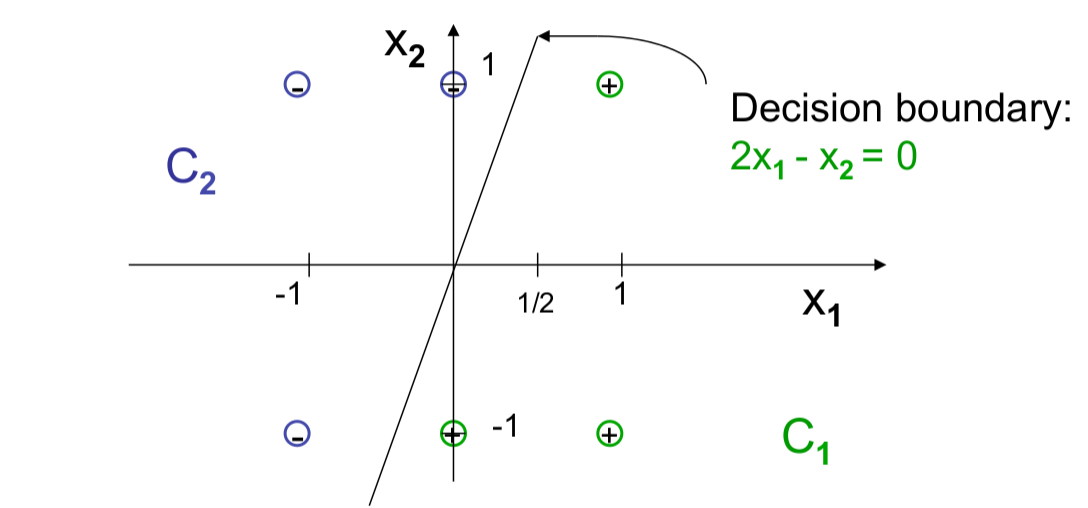
\includegraphics[width=0.6\textwidth]{bias1}
\end{figure}

To have the example actually use the bias the data can be modified: offset by (1,0). In this case the decision line would have to not go through the origin but the classes would remain linearly separable.
To validate the provided percepton learning algorithm the bias is added to the inputs and they are introduced to the perceptron.


\begin{table}[htb]
\centering
\label{bias_data_1}
\begin{tabular}{|c|c|}
\hline
\textbf{C1} & \textbf{C2} 	\\ \hline
	(2, 1)	&   (0, 1)		\\ \hline
	(2, -1)	&	(0, -1)   	\\ \hline
    (1, -1)	&   (1, 	1)		\\ \hline
\end{tabular}
\end{table}



\begin{table}[htb]
\centering
\label{my-label}
\caption{Epoch 1}
\begin{tabular}{|c|c|c|c|c|}
\hline
\textbf{Adjusted pattern} & \textbf{Weight applied} & \textbf{w(n) x(n)} & \textbf{Update?} & \textbf{New weight} \\ \hline
(1, 2, 1) & (1, 0, 0) & 1 &  No &  (1, 0, 0)  \\ \hline
(1, 2, -1)& (1, 0, 0) & 1 &  No & (1, 0, 0) \\ \hline
(1, 1, -1)& (1, 0, 0) & 1 & No & (1, 0, 0) \\ \hline
(-1, 0, -1)& (1, 0, 0) & -1 & Yes & (0, 0, -1) \\ \hline
(-1, 0, 1) & (0, 0, -1)  & -1 & Yes & (-1, 0, 0) \\ \hline
(-1, -1, -1)&(-1, 0, 0) &  1  & No & (-1, 0, 0) \\ \hline
\end{tabular}
\end{table}

\begin{table}[htb]
\centering
\label{my-label}
\caption{Epoch 2}
\begin{tabular}{|c|c|c|c|c|}
\hline
\textbf{Adjusted pattern} & \textbf{Weight applied} & \textbf{w(n) x(n)} & \textbf{Update?} & \textbf{New weight} \\ \hline
(1, 2, 1) & (-1, 0, 0) & -1 &  Yes &  (0, 2, 1)  \\ \hline
(1, 2, -1)& (0, 2, 1) & 3 &  No & (0, 2, 1) \\ \hline
(1, 1, -1)& (0, 2, 1) & 1 & No & (0, 2, 1) \\ \hline
(-1, 0, -1)& (0, 2, 1) & -1 & Yes & (-1, 2, 0) \\ \hline
(-1, 0, 1) & (-1, 2, 0)  & 1 & No & (-1, 2, 0) \\ \hline
(-1, -1, -1)&(-1, 2, 0) &  -1  & Yes & (-2, 1, -1) \\ \hline
\end{tabular}
\end{table}

\begin{table}[htb]
\centering
\label{my-label}
\caption{Epoch 3}
\begin{tabular}{|c|c|c|c|c|}
\hline
\textbf{Adjusted pattern} & \textbf{Weight applied} & \textbf{w(n) x(n)} & \textbf{Update?} & \textbf{New weight} \\ \hline
(1, 2, 1) & (-2, 1, -1) & -1 &  Yes &  (-1, 3, 0)  \\ \hline
(1, 2, -1)& (-1, 3, 0) & 5 &  No & (-1, 3, 0) \\ \hline
(1, 1, -1)& (-1, 3, 0) & 2 & No & (-1, 3, 0) \\ \hline
(-1, 0, -1)& (-1, 3, 0) & 1 & No & (-1, 3, 0) \\ \hline
(-1, 0, 1) & (-1, 3, 0)  & 1 & No & (-1, 3, 0) \\ \hline
(-1, -1, -1)&(-1, 3, 0) &  -2  & Yes & (-2, 2, -1) \\ \hline
\end{tabular}
\end{table}


\begin{table}[htb]
\centering
\label{my-label}
\caption{Epoch 4}
\begin{tabular}{|c|c|c|c|c|}
\hline
\textbf{Adjusted pattern} & \textbf{Weight applied} & \textbf{w(n) x(n)} & \textbf{Update?} & \textbf{New weight} \\ \hline
(1, 2, 1) & (-2, 2, -1) & 1 & No &  (-2, 2, -1)  \\ \hline
(1, 2, -1)& (-2, 2, -1) & 3 &  No & (-2, 2, -1) \\ \hline
(1, 1, -1)& (-2, 2, -1) & 1 & No & (-2, 2, -1) \\ \hline
(-1, 0, -1)& (-2, 2, -1) & 3 & No & (-2, 2, -1) \\ \hline
(-1, 0, 1) & (-2, 2, -1)  & 1 & No & (-2, 2, -1) \\ \hline
(-1, -1, -1)&(-2, 2, -1) &  1  & No & (-2, 2, -1) \\ \hline
\end{tabular}
\end{table}

If 4 epoch the algorithm converges to the line $2x_1-x_2=2$, the classes are separated, bias is nonzero.
The learning iterations on the adjusted patterns with added biases would be as shown in tables 1-4.

\end{document}
